\chapter{Model}  \label{chapter-model}
\epigraph{One of the very important components in the urban and agricultural land use model is the so-called \gls{bid-rent curve}. Regional and urban economists, city planners, and economic geographers have used this curve extensively as an analytical device.}{Yeung-Nan Shieh \cite{shiehWilhelmLaunhardtBidRent2004}}

% FUTURE WORK Because our goal  is to extend current model by introduce speculative motives and financialization, we retain the single-type household of the basic model, we defer the  question of the differential effect on household types for later work.  

%because a key feature of this model is that it formally captures how finalization works to capture the 
%financialization is aimed at capturing the 
%rents generated by growth and specifically urban growth..

% LINK WHAT TO WHAT..
% The feature of the model that provides the necessary link is known as the `\gls{bid-rent curve}.' We will incorporate  the  financial sector into  land market using the bid-rent curve.

%We begin in Section~\ref{section-financialize} with a definition of the act of financializing transactions and markets,  and discuss some significant examples. 

%Finally, in  Section~\ref{section-system} we explain how financialization might affect the housing market as a system and some consequences for society in general. 
%At that point we can introduce our specific hypotheses and how we intend to test them.
% We  focused on modelling the  effects of financialization on and through the urban housing market to \textbf{WHY?}. 
% This is where the general process of financialization At that point we can introduce our specific hypotheses and how we intend to test them.
% We therefore begin with a narrow and strict definition of the act of finacializing, followed by  an explanation and examples. We then go on to explain how the term is applied at the level of systems and while markets.
% At that point we can introduce our specific hypotheses and how we intend to test them.

% COULD CALL THIS THEORETICAL DEVELOPMENT OF THE MODEL AND MAKE A SEPERATE IMPLEMENTATION CHAPTER

% This chapter describes the specific formulations % (**E USE A MORE SPECIFIC WORD THAN LINKS) % #E BUILD A PCITURE OF HOW THE MODEL DRAWS THESE TOGETHER \dots LIKE IT TAKES THESE THREAD (LIST THEM) AND COMBINES THEM INTO A MODEL THAT EXPLORE \dots USE THIS PARRARAPH TO DESCRIBE THE EXACT INTERCONNECTIONS

% the theoretical discussions of the previous chapters with an agent-based simulation model. 

% At the heart of the model is a real estate mark et in which owners, tenants, new entrants to the city and non-resident investors participate. To do that we build up our model in a series of steps beginning with a notion of economic value, adding potential speculative gains, and finally describing a transaction process. %We need to specify the market process in more detail. (???) % i DONT UNDERSTAND IF YOU ARE SAYING YOU NEED THIS? THE MODEL FILLS THIS GAP?? OR THIS IS AFILLER SENTECEN??? 

% This chapter introduce the urban spatial model and labour supply, models the production function with urban scaling of agglomeration effects with density, then introduces a model of financial investment/speculation into a spatially explicit land market model, then calculates profit, considers who gets the profit, and draws conclusions. 



%     MOVE THIS?
%Recent urban models %, on the other hand, tend to focus on the locational implications of land and transportation costs on the location of people. Wealth distribution is  often ignored. 

% - need to  model production, specifically the rising production with density. 
%There is an extensive formal apparatus in economics for considering the relation of production and output. 
% \section{The general structure of the model}
In this thesis  we describe an agent-based spatial model of an urban housing market that includes a production function modelling how urban regions generate wealth and an explicitly financialized housing market.  Where previous chapters discussed general the principles that underlie our theoretical model, this chapter presents details about the how the variables in the computational model are defined. %Where, for example, we talk about expected price in Chapter~\ref{ch_financialization}, here we  provide the formula we use in our simulations.

% The model is introduced in the following sections:
% \begin{enumerate}
% \item In Section~\ref{sec_model_blocks} we  begin by describing the major blocks of the model. 

% \item In Section~\ref{sec_model_dynamics}  we make some comments on the dynamic properties of the model we have constructed. 

% \item In Section~\ref{sec_model_variables} we describe how a series of key  variables are constructed. The variables enter the decision-making process of agents in the market. 

% \item In Section~\ref{sec_model_bid_price}     

% \item In Section~\ref{sec_model_bargaining}    

% \item The treatment of time a periods and discounting is discussed in Section~\ref{sec_model_time}. 
%  Section~\ref{sec_model_price_expectataions}


% \item In Subsection~\ref{sec:Production-fn} we introduce the production function, introduce the labour supply and the urban model, the source of the surplus,  then we calculate profit, consider who gets the profit, and from there we draw our conclusions.. then we calculate the urban surplus, and consider who gets it. 

% \item Appendix~\ref{appendix-model-implementation} gives more details, describing the calculations, and showing how the model is implemented in code. 

% \end{enumerate}

% % % In subsequent sections  .. (Derivation details in Section~\ref{section-derivations})


% \section{The three major blocks of the model}\label{sec_model_blocks}

Our goal has been to make a model as accessible as the Alonzo model that can still provide insights about  the impact of financialization of the housing market on urban productivity and wealth distribution.  The  model has three major blocks:

{\newpage\thispagestyle{empty}
\vspace{-1.5cm}
\begin{figure}
\vspace{-1cm}
\begin{adjustwidth}{-0.24\textwidth}{-0.24\textwidth}
\centering
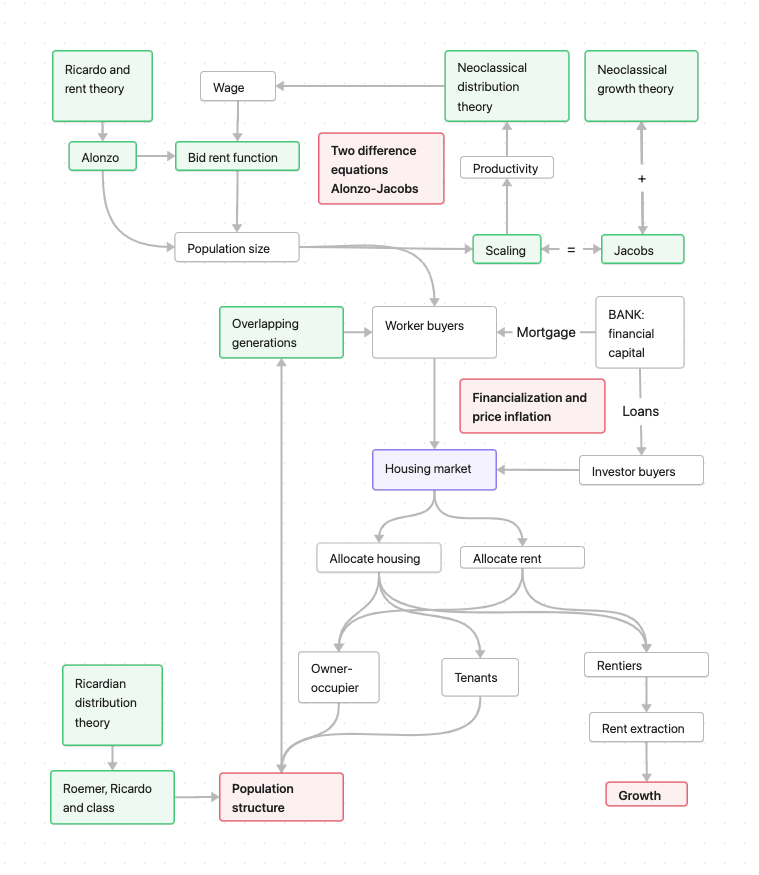
\includegraphics[scale=.6]{fig/flow-full-model.png}
\label{Stylized model flow.}
%\pagestyle{headings}
% \usetikzlibrary{positioning}
%\begin{tikzpicture}[remember picture,overlay,shift={(current page.north east)}] \node[anchor=north east,xshift=-1cm,yshift=-1cm]{\includegraphics[width=1cm]{example-image-a}};\end{tikzpicture}
\end{adjustwidth}
\caption{Model logic }\label{fig-flow-full-model}
\end{figure}
}

\begin{enumerate}
\item We incorporate the spatial structure of the city and its transportation system using a version of the \gls{bid-rent function} that drives all Alonso-style models. This equation is embedded in the decision of every agent because it determines the economic rent for each piece of property.

\item We incorporate the fundamental wealth production process of the city using an \gls{urban scaling} law that captures Jacobs-style agglomeration effects. This allows us to bypass the complexities of labour and goods market adjustments and instead to deal with the underlying long-term relationship between city population and production. We call the combination of this Jacob agglomeration effect with the Alonso model an \gls{Alonso-Jacobs model}. Together these two difference equations, operating on two aggregate variables, incorporate the major insight of a half-century of \gls{neoclassical growth theory}.

\item To link the Alonso-Jacobs model to the financial system, we develop an \gls{overlapping generations} model of the housing market with borrowers and lenders that tracks ownership and wealth. This turns out to be the most detailed and computationally-intensive part of the model. To model the effects financializing housing an \gls{agent-based model} we are forced to carefully specify the microeconomics of individual decisions. % In Section~\ref{section-micro},
We therefore, we describe the microeconomic objective function that individuals and our bank agent employ in deciding to purchase a property. 
\end{enumerate}

Figure~\ref{fig-flow-full-model} shows the model flow/logic.  The following three sections will discuss each of the three primary components, the spatial structure, the productivity mechanism, and the housing market in order.  To focus the model on the core questions of the relationship between urban productivity and rent, we keep the first two components,  the spatial structure and the growth mechanism,  as simple as possible, modeling the market for housing in more detail. 

% ANALYSIS???Finally, in  Section~\ref{section-system} we explain how financialization might affect the housing market as a system and some consequences for society in general. %At that point we can introduce our specific hypotheses and how we intend to test them.

\subsection{Spatial structure}

% In this section, we introduce the basic structure of the model, drawing on the circular city model.  
%  
% We build a spatially explicit agent model where agents work in one location and incur costs travelling to work. This work integrates a model of production and labour into a standard spatial model of the city. In this section, we introduce an analytic model of production and a labour market in a stylized circular city. 

% \subsection{Labour supply for production}
We begin with a model of a circular city. \footnote{In our computational model we use a grid structure with  a block metric, which is computationally more convenient and provides a slightly more natural representation of the property structure of actual cities.} %- INTRO CITY/APPROACH?
In the \gls{Alonso model} \cite{alonsoTheoryUrbanLand1960, alonsoLocationLandUse1964}, firms are located at the centre of a circular city, the central business district. Residents live distributed across space, can take jobs, and commute to work at the urban center. 
% In the simplest version, firms concentrate at the city centre. Workers are spread over space and pay transportation costs to commute.

Firms produce perfectly \gls{substitutable} % For simplicity, firms produce a variety of  goods, 
which they sell into a commodity market. Demand for the \gls{product} is \gls{perfectly elastic}, so the price remains constant. 

Firms purchase the time of workers. %to capture the product of their effective labour
%and enjoy the product of \gls{effective labour} . They can produce more goods by hiring additional workers. 
With the neoclassical model of distribution,\footnote{Clark's neoclassical assumption \cite{clarkDistributionWealthTheory1899}.} 
% We assume that the neoclassical model of distribution holds in the long run and 
workers receive the value of their marginal product. 

% TODO this shows the dynamics of a local economy, trade dynamics dominate local dynamics in many cases, that is explored with the addition of more cities and centres. 
 
%NEED TO INTRODUCE SUBSISTENCE WAGE BEFORE MENTIONING IT ABOVE %[MAYBE This follows xyz's approach, and makes it possible to explore resident's choice to work]. 


As in the Alonso model, described in Chapter~\ref{chapter-space}. The {urban wage premium} and transportation costs together determine both the radius of the circular city and the size of the labour force, %?There is no fixed boundary and the size of the city is determined by the utility that can be achieved in competing regions of competing for labour.
% and as in the standard circular city model the constraint on growth is provided by transportation costs, which limit the size of the commuter-shed and therefore the labour force at any wage. 
 %The raidus of the commuter shed is thus,  %The farthest workers will travel to work is thus 
% The  productivity of the city attracts people. 
since agents work if the wage premium is greater than the cost of travel. % Living close to work has value to workers because it saves the cost of transportation. 
The higher the wage, the  farther workers will commute. %This is the core of the Alozo circular city model.
The farthest workers will travel  is $\frac{w}{{c}}$, where ${c}$ is the cost of transportation per unit distance. This defines the radius of the city and the commuter shed.

The \gls{urban labour supply} is an \gls{aggregate} measure that emerges from individual agents' choice to commute. Considering a \gls{circular city} with a uniform lot size, $s$, with one worker per unit land, for illustrative purposes, the labour available is simply the area of the circle divided by the lot size: 
\begin{equation}
%=  \frac{\pi}{s}(c^{max})^2	
 L = \frac{\pi}{s} \left(\frac{w}{{c}}\right)^2
   =\frac{\pi}{{c}^2 s} w^2,
\label{eqn-labour-supply1}
\end{equation}
In an equilibrium analysis, this would be the equilibrium \gls{urban labour supply} curve, our version of the standard urban \gls{migration equilibrium} condition for models of this class. %which is a \cite{GET_migration_equilibOR_pop_equilib_condition}. %It defines the quantity of labour available.

%\footnote{See the discussion of model extensions in Appendix~\ref{appendix-future-work}.}.
% To get the \gls{urban wage premium}, we can write the inverse of the labour supply function:
% \begin{equation}
% w= (\frac{ {c}^2s}{\pi})^{0.5} L^{0.5}.
% \label{eqn-inverse-labour-supply}
% \end{equation}

\subsection{Agglomeration and productivity}\label{sec:Production-fn}

% *** ADD BACK? To study the productivity of cities, we incorporate Jacobs-style agglomeration economies (\cite{beaudryWhoRightMarshall2009, vanderpanneAgglomerationExternalitiesMarshall2004, jacobsEconomyCities1969}), using an approach similar to the way the \gls{Solow-Swan model} incorporates labour-augmenting technical change with a \gls{Cobb-Douglas} production function, and building the production function into a standard Alonso-style model of an urban economy.
%, using a simple Cobb-Douglas production function. 
% We incorporate the estimated scaling relationship in 
%The scaling result at the level of the city allows us to incorporate the agglomeration effect in a \gls{circular city} model, 
There is an agglomeration effect that augments the productivity of workers. This means firms produce more goods with a given stock of labour if the city is larger and urban workers are more productive, % than rural workers due to the positive agglomeration externalities. 
so urban firms can pay a premium to attract workers, that depends, among other things on the size of the city. % , above the subsistence wage.
%in a city with more people, as introduced in Chapter~\ref{chapter-growth} on growth.(**E SEE NOTE HERE) % #E i THINK YOU NEED TO FLESH THIS OUT, i'M NOT SURE EXACTLY WHAT YOU ARE SAYING. JUST BE A BIT MORE SPECIFIC AND FLESH OUT. 
% \subsection{Labour force}
%There are also firms that produce goods to sell. (???) % #E HOW IS THIS DIFFERENT THAN THE FIRMS PRODUCING GOODS IN THE PREVIOUS PARAGRAPH???

% Firms sell the goods they produce into a commodity market. 
 %, which are both exported and locally consumed 
% to sell into a large market, at a fixed price. 

To focus the model on urban productivity and the growing urban wage premium, we model workers as receiving a \gls{subsistence wage} $\psi$ in the countryside. Classical economists employed the \gls{subsistence wage} assumption to simplify their analysis in a similar way \cite{GET_classical-subsistence-wage}. This subsistence wage could come from work in the local community, living off the land, family support, social support, or something else. 
 % The model is set up so that all of an urban  tenant's  income is spent on  basic living costs, $\omega$, transportation $td$ or rent. Disposable income for owner occupier $i$ is therefore just the return  $\omega -dc$ which may accumulate as a financial asset.
% To attract workers to live in the city and commute to the central business district, firms pay the  \gls{urban wage premium}, $\omega$, in addition to  the subsistence wage $\psi$. 
%\footnote{See parameter appendix Section~\ref{section-wage-premium} for a discussion of the empirical literature on the \gls{urban wage premium}.}. 
% When workers take a job, they give up the subsistence income and, % instead receive a wage from their employer. % When workers take a job, they  receive, in addition to the subsistence wage,  the wage premium  from their employer. 

Urban workers give up the subsistence income and receive the \gls{urban wage}, $\psi +  \omega$, the subsistence wage plus the \gls{urban wage premium} that firms pay to attract workers. 
% When we assume an subsistence wage with a specific share  applied to housing we are implicitly assuming that landlords are seeking to claim the value of the rents. It makes it possible to explore whether and how tenants and even owners may be squeezed towards a \gls{subsistence frontier}. %whatever value the can. % tenants are squeezed by landlords. % DOES THE 'THIS' REFER TO THE FORMALIZATION OF WARRANTED RENTS?


According to \gls{neoclassical distribution theory}, the firm maximizes profit by setting the marginal value of the product of each \gls{factor of production} equal to the unit cost per factor. This means the wage premium increases in the same relation to population as \gls{productivity} does:
\begin{equation}
\omega\propto N^{\beta-1}.
\label{eqn-wage-population}
\end{equation}

% The city has single firm facing a fixed price for output. 

% IS THIS DUPLICATION? I THINK THE Solow-Swan model IS INTRODUCED IN SPACE CHAPTER. MOVE THIS TO SPACE CHAPTER IF NEEDED?
% In the \gls{Solow-Swan model}:
% \begin{equation} 
% Y(t) = K(t)^{\alpha}(A(t)L(t))^{\beta}
% \label{eqn-solow-swann}
% \end{equation}
% where $Y$, $K$ and $L$ are aggregate output, capital, and labour, respectively,  $A$ is the term the Solow-Swan model introduced for technology. The technology term capture the growth of labour productivity over time, $\alpha$ is the \gls{elasticity} of output with respect to capital, $\beta$ the elasticity of \gls{output} with respect to \gls{effective labour}, and $t$ time. If $\beta=1-\alpha$, this is a \gls{constant returns to scale} \gls{CRS} production function at the firm level.
% In the Solow-Swan model all factors of production are fully employed, and initial values $A(0)$, $K(0)$, and $n( 0 )$ are given. The number of workers, i.e. labour, as well as the level of technology grows exogenously at rate %s are $n$ and it   $g$,% respectively:  $L(t)=L(0)e^{nt}$     $A(t)=A(0)e^{gn}$ 
% This model uses a similar functional form to look at the effect of population density increasing % productivity. %how density increases in in  % It models how population increases productivity. 

The urban wage premium scales with the agglomeration effect. The \glspl{agglomeration effect} ensure urban \gls{output} is more than proportional to urban population: 
 \begin{equation}
 Y\propto N^{\beta},
 \label{eqn-production-population}
 \end{equation}
where $\beta$ is the elasticity of output with respect to capital, $\beta > 1$ where the agglomeration effect is positive. % Setting $\beta = 1$ would be the \gls{constant returns to scale}. $\beta - 1$ is the extra return that comes from adding to people the city. That return is the agglomeration effect that belongs to the city, it could go to the people.

We can put this together using a model of the production function. We implicitly use a three-factor model of \gls{production}, where production, is a function of capital and labour as well as a third factor, a Solow-Swan style term for labour augmenting technical change, with an \gls{agglomeration} effect, $A(N)$, in place of technology, $A(t)$. Output is:

\begin{equation}
Y=A(N)K^{\alpha }(A(N)N)^\beta.
\label{eqn-prod1}
\end{equation}
where $K$ is capital, $\alpha$ is the elasticity of output with respect to capital, $\alpha = \beta - 1$, and  $n$ is the \gls{urban labour supply}. $A(N)$ incorporates Jacob-style agglomeration externalities. $A(N)N$ is \gls{effective labour}.\footnote{The function  was discussed in Chapter~\ref{chapter-growth}.}

% \section{Agglomeration Appendix: Production Function}
% SORT APPENDIX/OTHER STUFF

% The agglomeration factor increases with population. It multiplies labour because agglomeration scales the productivity of workers.  
% It is a model of a productive urban economy since the centre is productive and demands labour.
% The growth of population feeds back into productivity. % We allow rising population to directly increase the wage.  
% We supplement the spatial model with agglomeration effects consistent with the literature. % in the base model. 
% There is an agglomeration effect, which
% The agglomeration effect means firms can also produce more goods by operating in a city with more people, because of the connections and interactions between people (CITE). 
 
 %, we assume the presence of scaling, consistent with neoclassical growth models as discussed in Chapter~\ref{chapter-growth}. 
%In this section, we introduce the basic structure of the production side and connect it to the literature on urban scaling. 
% We bypass the complexity of modelling firms, allowing population increases to directly increase urban wage premium.
%, It is straightforward to compute the rate of excess return for  this model. 

% We assume that the firm behaves as a price taker in the labour market as well, despite the fact that we model it as a \gls{monopsonist}\footnote{}. JUSTIFY/REPHRASE/EXPLAIN monopsonist. %ALSO DOES THIS GO HERE OR BELONG WITH PRIOR SECTION?

% Labour demand is thus a derived demand based on standard neoclassical theory with an equilibrium wage offer that is the marginal (value) product of labour for the firm. Specifically, hiring proceeds until the marginal product of labour is equal to the wage.

% The firm adjusts its labour force upward when the \gls{marginal product of labour} is greater than the wage by selecting from its list of job applicants.
% The firm adjusts its wage offer upward when the marginal product of labour is greater than the wage and it faces a labour shortage.  Labour shortage is a situation where the firm wants to hire but its list of job applicants is empty.

% The marginal product of labour is monotonically declining, ensuring a labour market equilibrium, to connect with the analytic tradition of economic modelling by ensuring there is an equilibrium level of production.  While adding more labour may always adds some value, the rate at which it adds value drops off. 
% If the marginal product increased, then a firm that got large enough would out compete smaller firms, hire all labour, always be able to produce more wealth by hiring more people, and would always produce more wealth by hiring people than by firing people. This doesn't happen. 
% Perhaps, the firm hires employees who best fit its needs first, but to grow, eventually it must hire less selectively. Finding markets may get harder with growth. Perhaps expansion adds additional costs, building a parking lot, administration, acquiring a larger building. Whatever the explanation, the marginal product of labour declines. 

% Frictional unemployment usually just refers to people moving between jobs. When people look for jobs, it may take time to get them. The analytic model offers an equilibrium solution with full employment. In the agent-based model this assumption does not hold, workers are laid off, and take time to find new employment.
% labour adjustment costs include moving costs for the employee or hiring, firing, or training cost for the firm. (there might be a hiring, firing, or training cost on the firm side, or on the employee side: expected time to employment costs, moving costs, etc.)
% The assumption of monotonically embedded marginal product of labour is embedded in the production function, so it applies in the analytic and agent models. This appears in the requirement that the sum of the exponents in the \gls{Cobb-Douglas} are less than one without agglomeration effects. Agglomeration effects can push the sum above one. When the exponents add up to less than one, there are diminishing returns to scale.  Exploring alternatives would involved exploring other formulations of the production function.

% $mvp(x) = p(x)$ where x can be labour, capital or any other factor, falls out of the function when you introduce profit maximization. Continuity and differentiability assumed but it is a convenient approximation-- take away assumptions you typically get a close approximation.

% We have a two factor model of production with labour and capital.  

\subsection{Financialization} 
%Our goal is to look at the relationship between urban production/labour markets, agglomeration, and land/housing markets. To explore this relationship we build a simplified model of a \gls{housing market}.% CALL IT LAND, PROPERTY, OR HOUSING MARKET? % - it is the housing use, combined with location we're interested in. % we introduce a \gls{land market}.% Agents purchase homes though a housing market. 

% In cities, housing is exchanged on a market. The product is properties, whether they're apartments, or land with the buildings on it. Properties have features including building size, style, quality, and location  that affect their desirability. %the buildings have a particular size and characteristics. %with various buildings and features. %properties on them. 
%Location also matters, %Land value  is affected by various elements
%including proximity to natural features like lakes and mountains, and human-built features like communities, and businesses, as well a developments and additions on the property itself. 
%Thereal market invovles  a set of agents who engage directly like buyers, sellers, renters, investors, and developers; as well as others who shape the market indirectly, including policymakers, activists, and neighbourhood and industry groups.
%The actors work within the context of a layer of policy, institutions, and rules. For example financial institutions offer debt, zoning allows certain uses and disallows others, and tax rules shape financial returns.

% and charges taxes and fees which are factored into the cost structure.
% shapes the land value.
% Our simulation model extracts % #E IS THIS A TECHNICAL TERM? i DON'T KNOW WHAT IT MEANS? yOU USE THESE TOGETHER. IF ITS STANDARD USAGE IGNORE THIS COMMENT
% these features to explore a core set of questions about financialization in land markets, in a way that's extensible to study a broad range of questions about real/particular markets in particular places.
% We study \gls{financialization} in a simplified market model, integrating
% In the simplified market model, %  owners sell when the retire.
% we integrate the % spatially explicit property market
% our urban production model  into a spatially explicit {housing market} with financial investment. %\gls{financialized} investment.

%Urban productivity drives land values through the housing market. Where there is a strong labour market, residents have a greater willingness to pay for housing \cite{GET_productivity_price_link} %ELABORATE. 
% Other factors also shape prices, including \gls{amenity}.

% *** In the model, rising \gls{population} and \gls{productivity} generate an economic value for land, that's derived from its proximity to the \gls{urban center}. 

% Use of a unit of land in each cycle is valued at the wage premium net of transportation costs. 
 % A worker, located at a distance $d$ from work, paying as much as $w- {dc}$ in rent, would still choose to work.

%\subsection{The microeconomics of  financialization} \label{section-micro}

Financialization happens at this microeconomic level, where individual decisions are made and real assets are bought by individuals and institutions. 
Properties have features including building size, style, quality, and location that affect their desirability. 
Agents exchange properties on a market,  
% Individual home-buyers are buying a stream of housing services and possible capital gains. Institutional buyers are buying 
and the return on housing as an investment is part of all agent's decision process. 
Private homeowners live in the properties they purchase, so when they purchase a property, they are buying both a stream of housing services and potential capital gains. %When a home is bought to live in, the potential buyer %makes a similar calculation, perhaps with a 
They may place particular emphasis on the value of the stream of housing services that matter to them individually. When home prices rise rapidly, speculative gains may become the dominant concern of home buyers. 
Investors, on the other hand, buy a stream of net rents plus speculative gains.
Each agent has their own interest rates, discount rates, mortgage share, information, and expectations, so individual bids can differ. 
%In the process, the real asset takes on an additional and separate aspect as financial object that can be bought and sold.  % The feature that matters most to investors is the  \gls{rate of return} that  an asset offers. 

Capozza et al \cite{capozzaFundamentalsLandPrices1989} show that land price has four additive components: the value of agricultural land rent, the cost of conversion, the value of accessibility, and the value of expected future rent increases. The first two can be treated as a constant.\footnote{Section~\ref{sec-extensions-conversion}, in Appendix~\ref{appendix-future-work}, discusses the potential for more detailed modelling of the land assembly and development process.} The third and fourth are the focus of this work. The value of accessibility in our model is determined by the urban wage premium, which rests on the productivity of the city. Expected future rent increases are driven by increases in the value of accessibility, which is to say, the rising productivity of the city. Productivity rises in our model due to pure agglomeration effects. Our concern is with what happens to the city and its people when financial capital captures the growing value generated by the agglomeration process.  

% For any level of risk and liquidity, an investor will choose to purchase the asset with the highest expected rate of return. 
To model the investment decision  we calculate the \gls{rate of return} on each property taking into account the rental revenue, the potential capital gain, the investors' costs of capital, incomes, and assets. The analysis will show the incentive structure driving the  financialization of the housing market. We do this in detail in Appendix~\ref{appendix-bid-price} 
The model must  allow for bidding and speculative investment but also must reflect the underlying economic value driven by urban productivity. To calculate the \gls{rate of return} we, therefore, need to define the relevant variables, and make some distinctions among different notions of rent and price %, including a variety of prices perceived prices  bid price3s

% \section {Variables}\label{sec_model_variables}


\section{Rent} \label{section-rent}
The explicit treatment of rents and the relationship between the productivity \gls{premium} and the \gls{subsistence wage} is what makes this a \gls{classical} model. 
% Rents go to the owners of a given property. If workers own their own homes, rents go to them. If others own the land, they can extract the rent. 
%In each period a house offers two kinds of services: {locational services} or  access to the central city job and amenities, and {home services}.  The {warranted rent} is the value of a complex stream of services. 

% *** TABLE ALSO NEEDS NET RENT $\mathcal{R}_N$ - WE SHOULD THINK ABOUT BEST WAY TO COMMUNICATE RELATIONSHIPS BETWEEN RENT TERMS.
\begin{table}[!ht]
\centering
{\renewcommand{\arraystretch}{1.6}
\begin{tabular}{r|c|c|c|c|c|c|c|}\cline{2-8}
       & Warranted  & Market & Expected & $i$'s Expected & Reservation & Asking & Bid     \\ \cline{2-8}
Price  & $P_{W_j}$      & $P_{M_j}$  & $P_{M_j}^\epsilon$ & $P_{M_{ij}}^{\epsilon}$     & $P_{R_{ij}}$       & $P_{A{ij}}$  & $P_{B{ij}}$   \\ \cline{2-8}
Rent  & $\mathcal{R}_{W_j}$      & $\mathcal{R}_{M_j}$  & $\mathcal{R}_{M_j}^\epsilon$ & $\mathcal{R}_{M_{ij}}^{\epsilon}$     &       &   &   \\ \cline{2-8}
% Rent $\mathcal{R}_W$ & $\mathcal{R}_W$ &        &       &             & $\mathcal{R}_M$ &          &               \\ \cline{2-8}
\end{tabular}
 }   
\caption{Price and rent notation}
% \caption{Price and rent notation\protect\footnotemark} % https://tex.stackexchange.com/questions/10181/using-footnote-in-a-figures-caption
\label{table-price-notation}
\end{table}
% There are three pieces to this analysis: there's the warranted price based on the underlying economic value of living in a property, the link here with urban productivity, there's the biding and negotiation process, and then there's the realized market price. 

To develop the analysis, we track the quantities, outlined in Table~\ref{table-price-notation}.\footnote{In the table, we include indices for agent $i$ and property $j$, for clarity. In the following development we'll only use the subscripts where needed to distinguish between agents and properties.}

In the model, agents learn or set these values with the support of a real estate agent, and based on information provided by their bank about lending rates, etc. After setting prices, agents engage in a negotiation process. 

The link with urban productivity is made through the land rents distributed through wages and available for distribution. If agents own their own property, they capture the rents. If others own it, they capture the rents.

\subsection{Warranted rent} \label{section-waranted-rent}
We anchor our housing price expectations in \gls{warranted rent}. It is the maximum rent that could be extracted from tenants for the stream of services provided by location and the housing supplied. A higher level of rent would convince tenants they are better off leaving the city.
\footnote{The warranted rent can be thought of as a kind of \gls{attractor} or \gls{equilibrium} towards which prices evolve, abstracting %. Including it in the model introduces a long-run equilibrium value, rather than modeling 
the adjustment process. % independent of the tendencies of the market.  
Combining a model of long-run attractor dynamics with distributed agent interactions, combines the advantages of agent-based modeling and standard \gls{classical} and \gls{neoclassical} economic analysis to give insight into the dynamics of financialization. Chapter~\ref{chapter-methodology} on methodology discusses the approach.} 

Warranted rent includes three distinct streams of services, the value of access to employment, which we call economic rent, locational amenities, and housing services.

\subsubsection{Locational economic rent} \label{section-economic-rent}
The \gls{economic rent} is the value of surplus that arise from access to jobs in the centre of the city where agglomeration economies generate a wage premium. These are represented as %, on an annual basis, 
the wage premium, $\omega$, minus the transportation costs, $c$, for a property a given distance, $d$, from the center:

\[\omega - {dc}.\]

\subsubsection{Locational amenity} \label{section-locational-rent}
The warranted locational rent includes  the economic rent as well as a locational amenity, $\mathbb{A}$. Locational amenity includes very local site-specific amenities like access to schools or views, as well as a general urban amenity function that is the value of living in a particular location $\mathbb{A}$. For most of the discussion in this chapter we ignore locational amenities, although we make provision for them in our computational model.

\subsubsection{Housing services} \label{section-housing-services}
Housing services $\mathcal{H}_j$ are  tied to a particular property. They include the value of features like a building having a certain number of rooms, particular finishes, or landscaping, extensions or upgrades. To maintain our focus on locational rents, we simplify, fixing %the value of housing services, setting 
the value of the stream of housing services to a fraction $a$ of the subsistence wage, $a\psi$.

\subsubsection{Combined equation}
Combining the three streams, the economically \gls{warranted rent}, $\mathcal{R}_W$, is then: 
\begin{align}
\mathcal{R}_W=\omega - {dc} + \mathbb{A} + a\psi.
\label{eqn-warranted-rent}
\end{align}

\subsection{Market rent} \label{section-market-rent}
The \gls{market rent}, $\mathcal{R}_M$, is what agents actually pay. The market differs from the economically warranted rent as investors make individual decisions about rents, setting rents based on market conditions and their own expectations. 

As an initial approximation, we simplify, using the warranted rent to approximate the market rent:
\[\mathcal{R}_{M, 0}= \mathcal{R}_W.\] 
As the simulation continues the market price is the price realized through the agent based housing market mechanism, so it diverges from net rents.

\subsection{Net warranted rent} \label{section-net-rent}
Owners receives, not the total warranted rent, but the \gls{net rent} after expenses, including maintenance, taxes, and the cost of financing. The following sections detail the computation of each expense, and their combination into the net rent calculation.

\subsubsection{Annual taxation}
Owners pay property taxes based on appraised price, $P_{\tau}$:
\begin{align*}
\mathcal{T} &= \tau  \mathcal{P}_{\tau}.
\end{align*}
 
Where $\tau$ is the municipal tax rate or \gls{mill rate}, and the \gls{appraised value} is based somewhat approximately, and with a lag, on the \gls{market price}, so $\mathcal{P}_{\tau}$ is some fraction of $\mathcal{P}_{M, t-n}$.

\subsubsection{Annual maintenance}
Annual maintenance costs apply to buildings and lands but not to locational value, so it can be modelled as a share, $b$, of the housing services costs, $a \psi$: 
\begin{align}
\mathcal{O} &= a b \psi.
\end{align}

\subsubsection{Combined equation}
Combining, the \gls{net rent} is:\footnote{This is the net warranted rent. Market rent, $\mathcal{R}_M$, can be decoupled from this for many reasons. For instance, agents who have purchased a house, may be able to pass a share of financing costs through to tenants as part of the market rent, depending on market power. Some  migrants may accept lower utilities or may have access to higher wages. The market rent could include an additional term, $F(v, rM)$, where $F$ is a function of financing costs that depends on %how tight the market is, 
vacancy, $v$, financing costs, $r$, and the size of the mortgage to be financed, $M$. When all financing costs are passed on the tenant effectively buys the property for the investor. The market rent is what an investor would use for price setting, however we are short-cutting the rent price formation process with a long-run equilibrium approximation based on the rents that can be extracted before people leave the city, so the mechanisms that push rent up to that extraction value are abstracted and we work with the net warranted rent in the price formation model. There would be a strong feedback from speculators taking on financing costs  to the level of rents for tenants, and this  then feedback into prices. % These are distinct logics for the rent formation mechanism which can be explored through more explicit models of rental markets. Abstracting them gives a set of easily generalizable simplifications.% The way housing financing costs are passed through to tenants. are computed are detailed in the next sections.
% 
Annual financing costs are $rM$. 
}
\begin{align}
&= \mathcal{R}_W - \mathcal{O} - \mathcal{T}.
\end{align}

\section{Prices}
Even when all  housing units are identical except for location, there are several prices  to consider, including bid prices, reservation prices and expected prices. We will begin by considering  housing as an providing a flow of services, discuss expected prices and then go on to develop the bid price and the reservation prices for investors. 

A bidding process determines an actual realized market price, with bidders taking into account potential capital gains. We describe the bid price formulation below. 

To calculate agent bid prices, we first calculate the net present value of the purchase, then divide by the capital employed, which we assume is the size of the down payment made at the beginning of the period. This gives us a rate of return.\footnote{A common approach would be to calculate an internal rate of return (IRR), but  the IRR is in general the solution to a polynomial and does not guarantee a single-valued result \cite{robinsonOptimalTerminationIRR1996}. Multiple real-valued  IRRs may arise;  complex-valued IRRs may arise;  the IRR is, in general, incompatible with the net present value (NPV) in accept/reject decisions; the IRR ranking is, in general, different from the NPV ranking; the IRR criterion is not applicable with variable costs of capital. Ways to salvage the IRR as a usable criterion have been proposed that are consistent with our approach \cite{magniAverageInternalRate2010}, which is to calculate an NPV then convert it to a rate.} 
The rate of return on the investment must exceed some required rate of return. This condition allows us to calculate the maximum price that will satisfy that criterion.
% We assume that agent may be  speculating on potential \glspl{capital gain} as well as on the \gls{use value} or net market rent they get from the property. We therefore treat the purchase as an investment decision and compute a rate of return, $v$, conditional on the price paid. This allows us to 
We solve this for for the maximum bid, $P_{max}^{bid}$ that achieves the desired rate of return. 



\subsection{Price expectations}
The \gls{market price} or the price at which a property is exchanged on the market, $P_M$ will not be known in advance, nor will the future sale price.\footnote{Case and Shiller point out ``\dots we see a market largely driven by expectations. People seem to form their expectations from past price movements rather than having any knowledge of fundamentals. This means that housing price booms will persist as home buyers become destabilizing speculators''  \cite{caseThereBubbleHousing2003}. Case and Schiller\cite{caseThereBubbleHousing2003} argue that  the 1-year expectations are fairly well described as attenuated versions of lagged actual 1-year price changes.}  In order to make decisions, agent $i$ must form an \glspl{expectation} or prediction $P_{M_i}^{\epsilon}$ of an as yet unrealized future market price. Agent $i$'s expected market price may be affected by individual information, biases, preferences, and any assumptions the agent has about the behaviour of others, the system state.  


% The underlying value of a home is the capitalized value of the services it provides, which are perpetual.  Rents, however, depend on urban productivity and may change over time. Any expected increase in future rents capitalized into the market price of a home as a capital gain for the owner. Home prices should respond to expectations.

\subsection{Bid price}\label{sec_model_bid_price}
To model the market transactions when speculative motives are in play we need an expression for how much financial investors will bid. Specifically, we must find the maximum price that they are willing to pay. 
% As Horowitz \cite{horowitzBiddingModelsHousing1986} notes, a prospective buyer considering a vector of attributes of the property, including the seller's asking price and the property taxes, transaction costs, and financing costs at a specified price. The  potential buyer also is likely to have estimates of the maintenance costs and resale value of the house, although these may be highly subjective. All of these factors shape whether an investment is profitable. To make a comparison with alternative investments, it is necessary to compute a rate of return. 


    
 The agent who purchases makes a down payment, $D$ on a house for a price, $P_0$, and agrees to pay off a mortgage, $M$ with interest at the end of the mortgage period. For expositional convenience, we can treat the mortgage period $T$ as a single term and express all quantities  in present-value terms. The purchaser  receives the increased price $P_T = (1 + \dot P)^TP_0 = (1+\dot P^T)P_0$,  
 after a period $T$, Where $\dot P$ is the expected annual rate of price increase and we define $\dot P^T$ as the T-period  interest rate. The agent also receives either the net market rental value of the property throughout the period, $\mathcal{R}_N$, or if the owner is also the resident, the locational rents.

With a price-growth rate of $\dot P$ per year, the growth over $T$ years is $(1+\dot P)^T$, and  %and a 5 year mortgage period, 
the expected price at the end of the period is:

\[P_M^{Te}=P_0(1+\dot P)^T\]

If, for example price growth is 10\%, $\dot P= 0.1$, the {capital gain}, or growth, over a 5-year mortgage term is 0.61051 $\approx$ 60\% of the original price, $P_0$.

The rate of price growth, $\dot P$, is an approximation based on rents and past market behaviour. In our computational model we employ a regression model to generate an \gls{expected market price} based on past prices. The rate of price growth $\dot P$ we use in our model of investor behaviour is derived from the same regression model.

SOME REFERENCES - MOVE? \cite{anselinModernSpatialEconometrics2014, gelmanDataAnalysisUsing2006}.






{\color{blue}
 \subsubsection{The value of an investment}
% \subsection{The value of an investment}
The value $V$ of a property investment over a period of T years is  the capital gain, $P_{T}-P_{0}$, minus financing costs, plus net rent revenues. Both mortgage payments and net rent revenues can  be calculated as sum  of regular payments, each of  which accumulates interest to the end of the mortgage period. This is called a ``uniform series compound amount'' and is calculated for net rent as\footnote{Any annual payment for a period multiplied by the factor $\frac{(1+r)^n-1}{r}$ is called a  ``uniform series compound amount''.%source https://www.e-education.psu.edu/eme460/node/659
} 
\[\mathcal{\bar{R}}^T_N= \frac{(1+r)^T-1}{r}\mathcal{R}_N  \]
The regular mortgage payment is  $rM=rmP_0$,\footnote{we assume that the regular payment covers only the interest and that the full mortgage is due at the end of the period } and the uniform series compound amount is
\[\bar{rmP_0}^T= \frac{(1+r)^T-1}{r}rmP_0  \]
Both these amounts are discounted by $\delta^T$ to the present in our calculation.
 
 
% \[\mathcal{\bar{R}}^T_N=  \delta^T\frac{(1+r)^T-1}{r}\mathcal{R}_N  \]
% To keep the notation simple, let 
% \[\delta_r^T=\delta^T\frac{(1+r)^T-1}{r}\]
% The present value of the mortgage repayment plus the accumulated interest be 
% \[\bar M^T_r = \delta^T\frac{(1+r)^T-1}{r}\]
 We can write $V$ in terms of the purchase price, and several individual parameters: interest  rate, share of the price that can be mortgaged and  discount rate:%\footnote{The down payment could be deducted in advance, but if the discount rate is equal to the interest rate it drops out completely.}
 
 \begin{align}
V &= \delta^T\left( P^T-P_0- \left(\frac{(1+r)^T-1}{r}rM\right)- M+ \mathcal{\bar{R}}^T_N \right)      \\
&= \delta^T \left(
\dot P^T P_0 -\left((1+r)^T-1\right)mP_0-mP_0
 +  \mathcal{\bar{R}}^T_N \right) 
\label{first_sub}\\
  &= \delta^T \left(\dot P^T - (1+r)^T)m P_0 + \mathcal{\bar{R}}^T_N\right)
\end{align}
where $\dot P^T$  is the expected rate of change in the market price over the term of the mortgage.
$V$ is the net present value of buying and selling after one mortgage renewal period of $T$ years. %All rates are scaled to the length of the period to avoid the need for compounding calculations. 
The function has 4 individualized  parameters, $\delta$, $\dot p$, $r$, $m$, as well as any factors that affect the rent term.


{\color{red}

\subsubsection{Rate of return on investment}
We divide V by the size of the down payment, $D$ to get the  rate of return  

\begin{align}
r^{return} =
  &= \frac{V}{D}  \nonumber \\
  &= \delta^T \left(\dot P^T - (1+r)^T)m \frac{P_0}{D} + \frac{\mathcal{\bar{R}}^T_N}{D}\right)\\
  &= \delta^T \left(\dot P^T - (1+r)^T)m \frac{P_0}{P_0-mP_0} + \frac{\delta_r^T\mathcal{\bar{R}}^T_N}{P_0-mP_0}\right)\\  
  &= \frac{\delta^T}{1-m} \left(\dot P^T - (1+r)^T)m  + \frac{\mathcal{\bar{R}}^T_N}{P_0}\right)\\
\end{align}
Notice that the return depends on the price paid, $P_0$.


\subsubsection{Criterion for investment}
Equation~\ref{{eq:rate-of-return-on-investment}} provides a criterion for investors. Agents invest if  their expected return is greater than the target return, they are seeking:
\begin{equation}
r^{target}\le r^{return} 
\label{eqn-property-investment-return2}
\end{equation}

% We first calculate the net present value of the purchase, then divide by the amount of capital employed, which we assume is simply the size of the down payment made at the beginning of the period. This gives us a rate of return.\footnote{A common approach would be to calculate an internal rate of return (IRR), but  the IRR is in general the solution to a polynomial and does not guarantee a single-valued result \cite{robinsonOptimalTerminationIRR1996}. Multiple real-valued  IRRs may arise;  complex-valued IRRs may arise;  the IRR is, in general, incompatible with the net present value (NPV) in accept/reject decisions; the IRR ranking is, in general, different from the NPV ranking; the IRR criterion is not applicable with variable costs of capital. Ways to salvage the IRR as a usable criterion have been proposed that are consistent with our approach \cite{magniAverageInternalRate2010}, which is to calculate an NPV then convert it to a rate,} 

% Equation~\ref{eqn-return-on-investment} makes it clear that the estimated rate of return depends on subjective magnitudes,$\delta$ and $\dot P_M^e$, attributes of the property, $ \mathcal{R}_N$, and  individual financial position, $r$, $m$.
% 

\subsubsection{Maximum bids}
The maximum price in Equation~\ref{eqn-property-investment-return1} that the investor can price offer for the property  and still satisfy the inequality~\ref{eqn-property-investment-return2} $P_B^{max}$ is

\begin{align}
r^{target}& \le \frac{\delta^T}{1-m} \left(\dot P^T - (1+r)^T)m  + \frac{\mathcal{\bar{R}}^T_N}{P_B^{max}}\right)\\
% (1-m)r^{target}/\delta^T &\le \dot P^T - (1+r)^Tm  +   \frac{\mathcal{\bar{R}}^T_N}{P_B^{max}} \nonumber\\
% (1-m)r^{target}/\delta^T - \dot P^T + (1+r)^Tm &\le  \frac{\mathcal{\bar{R}}^T_N}{P_B^{max}}\nonumber\\
P_B^{max} &\le  \frac{\mathcal{\bar{R}}^T_N}{(1-m)r^{target}/\delta^T - \dot P^T + (1+r)^Tm}
\end{align}

% \begin{eqnarray}
% P_B^{max} & \le    \frac{\mathcal{\bar{R}}^T_N}{(1-m)r^{target}-\delta \left(1 + \dot P_M^e - (1+r)m\right)} \label{eqn-bid-price} \end{eqnarray}
% % P_B & \le    \frac{\mathcal{R}_N}{(1-m)r^{target}-\left[ \delta(1+L(P)- (1+r)m\right]}
We call this  $i's$ maximum bid and compute it for all potential buyers and sellers. In each sale the highest $P_B$ will make the purchase. The denominator can be seen as an adjusted rate of return for capitalizing net rents, analogous to the value of $r$ in  the standard capitalization formula.\footnote{We could allow potential buyers  to approach potential sellers who have not listed with an offer and allow worker-owners to consider retiring early or becoming tenants if an offer is attractive.  This is only likely if speculative pressures are strong. It may require having multiple institutional buyers to make offers more competitive. In that case, initial offers will be closer to the maximum bid price, tending to pull prices up and benefit potential sellers.}  
}
%Buyers will not initially bid the maximum and sellers will generally set an asking price $P^{ask}$ higher than their reservation price $P_R$, so we build a simple bargaining process.


\section{Reservation prices} 

Bargaining models attempt to identify the way the surplus available from a transaction is divided between the parties involved. The classic  formulation by John Nash %\cite{Nash_John% (1953-01-01). "Two-Person Cooperative Games". Econometrica. 21 (1): 128–140. doi:10.2307/1906951. JSTOR 1906951} 
identifies a `disagreement point,' which which is the  lowest value each player will accept. In bargaining over a price the lowest value for the seller is called the  `\gls{reservation price}.' The reservation  price for the seller is the highest amount the seller is willing to pay, which is the maximum bid price that we  have just calculated.  

 All owners and potential buyers have  reservation prices. They represents the owner's best alternative, and in bargaining models if the a maximum bid is higher than the reservation price the outcome is between the the two.  
\subsection{Seller's reservation price} \label{section-reservation-price}

We will assume,  that for owners, deciding to sell is a life-cycle decision. Home owners-workers  reach the end of their working lives, no longer need access to the central city, and put their homes on the market, making room for new workers to enter the urban market.%\footnote{The timing decision can be randomized, but that is highly unlikely to affect results.} 


If no sale is made the owner would consider becoming a landlord.\footnote{Worker-owners could remain in their homes after retirement. In that case,  there would be fewer homes available for new workers, which must produce a labour shortage in this model, driving up wages, and leading to higher bids and rising home prices, which in turn attracts  speculative bidding. This will only accelerate any shift in the ownership pattern. Our core model suppresses labour market dynamics and the effect of housing shortages to focus on the warranted prices, which are driven by aggregation economies.}  This would be a rational choice if the present value of net rent is above the the best selling price price. 
The value of the stream of rent is therefore the most reasonable reservation price. This stream must be discounted at the personal discount rate or at the personal borrowing rate.\footnote{As a further extension, worker-owners in the final few years of their working life might decide to list if they notice that the expected price posted by the real estate agent, $P_M^e$,  exceeds (say) 95\% of their reservation price. This is a `hopeful' listing, `fishing' for an offer that exceeds the actual reservation price.}


%
% \[P^{ask}>P_M^e> 0.95 P^r\]
% Otherwise
% \[P^{ask}> 1.10P^r>P_M^e\]
% If no offer exceeds the reservation price, no sale is made.

% Once an owner reached retirement age, if no sale is made the reservation price is reduced for the next cycle.
% If no sale is made the owner considers becoming a landlord. if the present value of net rent is above the reservation price, the owner rents out the home. 

\begin{figure}[!hb]
\centering
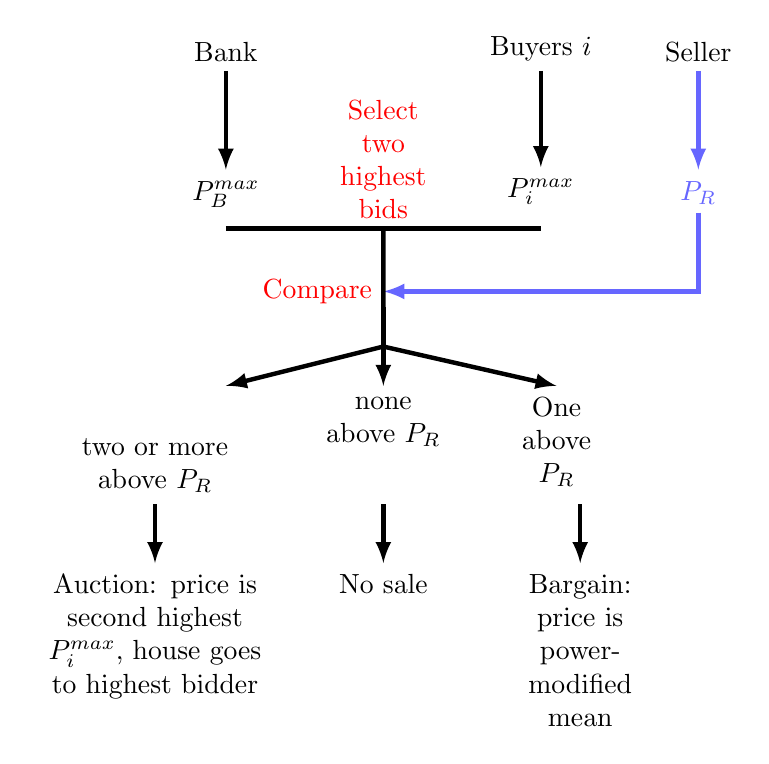
\begin{tikzpicture}
%\draw[step=0.5cm,color=gray] (0,-3) grid (8,7);
\node [above](Bank)at (1,7) {Bank};
\node [above](Buyers)at (5,7) {Buyers $i$};
\node [above](Seller)at (7,7) {Seller};

\draw[ultra thick, -latex](Bank)--++(0,-1.5)node[below]{$P_B^{max}$};
\draw[ultra thick, -latex](Buyers)--++(0,-1.5)node[below]{$P_i^{max}$};
\draw[ultra thick, blue!60,-latex](Seller)--++(0,-1.5)node[below]{$P_R$};

\node[above, red, text width=1.55cm, align=center]at (3,5){Select two highest bids};

\begin{scope}[shift={(0,-1)}]
\draw[ultra thick](1,6.)--(5,6.0); % Bar
\draw[ultra thick, blue!60,-latex](7,6.2)--++(0,-1)--++(-4,0)node[left, red]{Compare};  %Pass P_R to if-then
\draw[ultra thick, -latex](3,6)--++(0,-1.5)--++(-2.,-.5);% down and left
\draw[ultra thick, -latex](3,5)--++(0,-1)node[below, text width=1.5cm, align=center]{none above {$P_R$} };%
\draw[ultra thick, -latex](3,5)--++(0,-.5)--++(2.2,-.5)node[below, text width=1.cm, align=center]{One above {$P_R$} };
% down and Right

\draw[ultra thick, -latex](.1,2.5)node[above, text width=2.cm, align=center]{two or more above {$P_R$} }--++(0,-.75)node[below, text width=3cm, align=center]{Auction: price is second highest $P_i^{max}$, house goes to highest bidder};

\draw[ultra thick, -latex](3,2.5)--++(0,-.75)node[below, text width=2cm, align=center]{No sale};

\draw[ultra thick, -latex](5.5,2.5)--++(0,-.75)node[below, text width=2cm, align=center]{Bargain: price is power-modified mean};
\end{scope}

\end{tikzpicture}
\caption{The Bargaining model and price determination}
\label{fig:Bargaining}
\end{figure}
%We then check the initial bids and the asking price and apply a bargaining rule to determine how any surplus $P_B^{max}-P_R$ is allocated. The details of the bargaining rule will have little or no effect on the  behaviour of the system. 



\section{The bargaining model} \label{sec_model_bargaining}


\subsection{Many-to-many matching problem}
\textbf{We have a many-to-many matching problem}. Many buyers and sellers single sellers for each unit. Therefore, for each property that comes on the market each potential seller has a reservation price $P_{ij}^{reservation}$ and there will be a set\footnote{We could allow potential buyers  to approach potential sellers who have not listed with an offer and allow worker-owners to consider retiring early or becoming tenants if an offer is attractive.  This is only likely if speculative pressures are strong. It may require having multiple institutional buyers to make offers more competitive. In that case, initial offers will be closer to the maximum bid price, tending to pull prices up and benefit potential sellers.}  of potential buyers with maximum bids $P_{ij}^{maxbid}$.


This will appear in your data as a set of bids and a reservation price for each property on the market that must be converted to a price for that property using the bargaining rule. The rule is simple: 
\begin{enumerate}
    \item if there is only one maximum bid above the reservation price, split the difference.

    \item If there are two or more maximum bids above the reservation price, the property goes to the highest  and the price is the second highest
\end{enumerate}


\subsection{Another version}
In reality, sellers often post an asking price greater than the reservation price. All agents will expect to negotiate, however, so we assume instead that if there is a deal, it will result in a price between the bid and the reservation price, treating the higher asking price and bids as `cheap talk'\footnote{In game theory, cheap talk is communication between players that does not directly affect the payoffs of the game. Providing and receiving information is free. This is in contrast to signaling in which sending certain messages may be costly for the sender depending on the state of the world.} since a price outside of this range cannot be a rational choice for both sides, so it is ruled out in Nash bargaining theory.

The bargaining  mechanism then simply has to compare the maximum bid price $P_B$ with the seller's reservation price. If the $P_B^{max}>P_R$, a deal that is between the two values is possible. Otherwise, the transaction does not proceed.

If there are competing buyers with maximum bids higher than the reservation price, only the highest two need be considered. The second highest max bid should be the sale price, but the bidder with the highest max bid wins the property. This is realistic because in a bidding war the final bid only has to be a small amount higher than that of the last competitor left. That is the highest price that a seller can normally get.\footnote{This is an application of Vickrey \gls{second-price auction} theory. Bidders are asked to submit sealed bids. %b1, \dots 
The bidder who submits the highest bid is awarded the object, and pays the amount of the second highest bid \cite{levinAuctionTheory2004}.}

If $P_B^{max}>P_R$,  the bargaining rule selects a value 
\[P = xP_B^{max*}+(1-x)P_R\]
where $0\ge x\ge 1$ is approximately 0.5 but shifts upward when it is a sellers market and downward in a buyer's market.\footnote{In an overheated housing market bid prices might exceed asking prices, but the price wont exceed the maximum expected profitable bid price, $P_B^{max*}$.} We will call this term am measure of \gls{sellers' bargaining power}.  The sellers' bargaining power can be shifted downward if the home fails to sell in the first period it is on the market. 

\section{The process}
\begin{enumerate}
\item \textbf{identify the pool of sellers} for each cycle.
    \begin{enumerate}
        \item Agents who a) own and b) age out
        \item Agent  who failed to sell in the previous period.
        \item the bank
    \end{enumerate}
\item \textbf{identify the pool of buyers} 
    \begin{enumerate}
         \item newcomers, 
         \item individuals as investors.
         \item the bank may buy many, (There must be a capital (C) constraint something like $C/\bar P$ to select a number of bank bids in any period.)
    \end{enumerate}

\item \textbf{count buyers and sellers} and use the counts to identify sellers or buyers' market. \# Sellers > \# buyers is a buyers/ market. For a buyer's market  choose the lower price. \footnote{.The is often done with buyers/vacancies. Changes in this ratio are observed to trigger significant movement in rent r market prices.\cite{wheatonVacancySearchPrices1990}. Lisi and Iacobini \cite{lisiEstimatingHousingPrice2015} found  that in the Italian market, ``the difference between the actual selling price and the price obtained in an ideal situation of frictionless housing market – is remarkable. ... the higher the trading frictions on the demand side (more buyers and less sellers), the higher the actual selling price (the price adjustment is positive), whereas the higher the trading frictions on the supply side (less buyers and more sellers), the lower the actual selling price (the price adjustment is negative). '' (they point out that ``Trading frictions are obvious in the housing market, as it takes weeks or months to buy or sell a house (Caplin and Leahy, 2011; Rocheteau and Weill, 2011).'')}  

%a key role is played by the so-called “time-on-the-market (TOM)”. The time it takes to sell a property or “the expected time until the asset is sold when following the optimal policy” (Lippman and McCall, 1986) – commonly known as the TOM – measures the degree of illiquidity of the real estate asset and is a fundamental characteristic differentiating real estate from financial assets. \cite{lisiSearchMatchingProcess2019}
\item \textbf{The pooling problem}  Houses should go at different prices if they have different net rents.  Assume buyers and sellers are indifferent about location (no  local amenities) so only the net rent matters for the ban and only the full rent for individuals.

\item \textbf{Create lists} for the buyer pool and the seller pool. (The bank can appear on the list many times.) 

If the market is efficient, the allocation will maximize the sum or seller and buyer surplus.

\item To select the set of transactors, \textbf{order the lists}. Buyers from highest to lowest, sellers from lowest to highest.

\end{enumerate}


% Ensure that they are of the same length by dropping the lowest bids or the highest reservation prices. 

\newpage
\textbf{Possibly relevant Example of a matching problem drawn from game theory text}

There are 26  people, some with houses, Each values the house an amount equal to the last three digits of their student numbers. Those on the left of the table don't have a house when the game starts, indicated by a ``0'' in the second column. Those on the right  start with a horse, indicated by a  (1) in the fifth column and half don't. 

\begin{center}
Value and number of houses

\begin{tabular}{|c|c|}
 
\begin{tabular}{lcc}
max bid&start&end  \\ \hline
985  & 0 & 2 \\
829  & 0 & 1 \\
740  & 0 & 1 \\
650  & 0 & 1 \\
643  & 0 & 1 \\
611  & 0 & 1 \\\hline
532  & 0 & \color{red}1  \\
356  & 0 & \color{red} 1   \\
270  & 0 & \color{red} 1  \\
135  & 0 & 0    \\%69 & 1  & 0
   
\end{tabular}

&
\begin{tabular}{lcc}
reservation&start&end \\ \hline
 50 & 1  & 0 \\
127 & 1  & 0 \\
190 & 1  & 0  \\
245 & 1  & 0 \\
 324 & 1  & 0 \\
 522 & 1 & \color{red} 1\\\hline
 738 & 1  &  \color{blue}0 \\
 829 &1  &  \color{blue}0 \\
832 & 1 & \color{blue}0\\
   &  &              \\%69 & 1  & 0 
\end{tabular}

\end{tabular}
\end{center}


 
  \begin{tikzpicture}[scale=.8]
%  \draw [gray, opacity=.7]
 (0,0) grid (7,7);
\draw [<->] (0,10.5) node[above]{value}-- (0,0) -- (10,0) node[below]{Houses};

\draw [red, thick] (0,9.85)node[above right]{985}--(1,9.85)--(1,8.29 )node[above right]{829}--(2,8.29 )--(2,7.40 )node[above right]{740}--(3,7.40 )--(3,6.50 )node[above right]{350}--(4,6.50 )--(4,6.43)node[above right]{643}--(5,6.43)--(5,6.11)node[above right]{611}--(6,6.11)--(6,5.32)node[above right]{532}--(7,5.32)--(7,3.56)node[above right]{356}--(8,3.56)--(8,2.70)node[above right]{270}--(9,2.70)--(9,1.35)node[left]{DEMAND}node[above right]{135}--(10,1.35); 

\draw [blue, thick] (0,.50)node[above right]{50}--(1,.5)--(1,1.27 )node[above right]{127}--(2,1.27 )--(2,1.90 )node[above right]{190}--(3,1.90 )--(3,2.45 )node[above right]{245}--(4,2.45 )--(4,3.24)node[above right]{324}--(5,3.24)--(5,5.22)node[above right]{522}--(6,5.22)--(6,7.38)node[above right]{738}--(7,7.38)--(7,8.29)node[above right]{829}--(8,8.29)--(8,8.32)node[above right]{832}--(9,8.32)node[right]{SUPPLY}; 
%,2.5) ;
%\draw [blue, dashed] (0,4.5) node[left]{large bill}--(8.33, 4.5)-- (8.33,0)node[below] {large user Q};
%\draw [green, dashed] (0,0) --(8.33, 4.5);
%\draw [green, dashed] (0,0) --(1.66, 2.5);

%\draw [<->, shift={(7 cm,0)}] (0,6) -- (0,0) -- (5,0);
\end {tikzpicture}

The gain for any person is the difference between the transaction price  for a house and the amount they value a house




At the same time, for each p. NOT. DONE
\begin{eqnarray}
P_{bank}^{reservation} & \le  P_{person}^{max\_bid} \end{eqnarray}


% \begin{lstlisting}
% # parameters - max interest payment 
% max_mortgage_share = 0.28 # ability to cover a mortgage

% # Max mortgage

% wealth = property_value - mortgage + savings
% mean_weath = sum(wealth)/number_of_people

% def get_max_mortgage(self, applicant):
%     max_mortgage =  ...
    
%     return max_mortgage
% \end{lstlisting}




